\chapter{Lux.jl: Bridging Scientific Computing and Deep Learning}
\label{chapter:lux_bridging_scientific_computing_and_deep_learning}

% \citet{Rackauckas2020GeneralizedPL}

\section{Introduction}
\label{sec:introduction_lux}

\section{Composability via Generic Parameterization}
\label{sec:composability}

One of the distinguishing features of Lux.jl is its generic parameters interface. Lux can accept any special parameter type as long as the parameters are accessible via \textit{getproperty}. This allows Lux to seamlessly interface with packages that are completely agnostic to the specifics of Lux. This is in contrast to most prior works that require glue code for interfacing -- like Flux.jl~\citep{innes:2018} -- or requires reimplementing algorithms in specific Domain Specific Languages (DSLs) -- like Pytorch~\citep{paszke2019pytorch,paszke2017automatic}, JAX~\citep{jax2018github}, Tensorflow~\citep{tensorflow2015-whitepaper}.

Scientific Computing softwares differ from most modern ML softwares in that they are designed to operate on arrays, while ML softwares operate on deeply nested structures. This is a fundamental difference that makes it difficult to interface between the two. However, Lux.jl is designed to be agnostic to the underlying data structure. In this section we will demonstrate several examples interfacing Lux with packages completely agnostic to Lux.

\subsection{Neural Differential Equations}
\label{subsec:differential_equations_lux}

In this thesis, we have described Neural ODEs in great depth. However, for physics based modelling we often need to rely on higher order differential equations. In this section, we will describe how to model a second order differential equation using Lux.jl and OrdinaryDiffEq.jl. We will attempt to model the acceleration of a system using a Neural Network\footnote{We have modified this example from \url{https://docs.sciml.ai/SciMLSensitivity/stable/examples/ode/second_order_neural/}}:
%
\begin{equation}
  \frac{d^2u}{dt^2} = \texttt{NN}(u)
\end{equation}
%

\inputminted[linenos, breaklines, fontsize=\scriptsize, frame=single, framesep=10pt]{julia}{../code/diffeq.jl}

\begin{figure}[t]
  \centering
  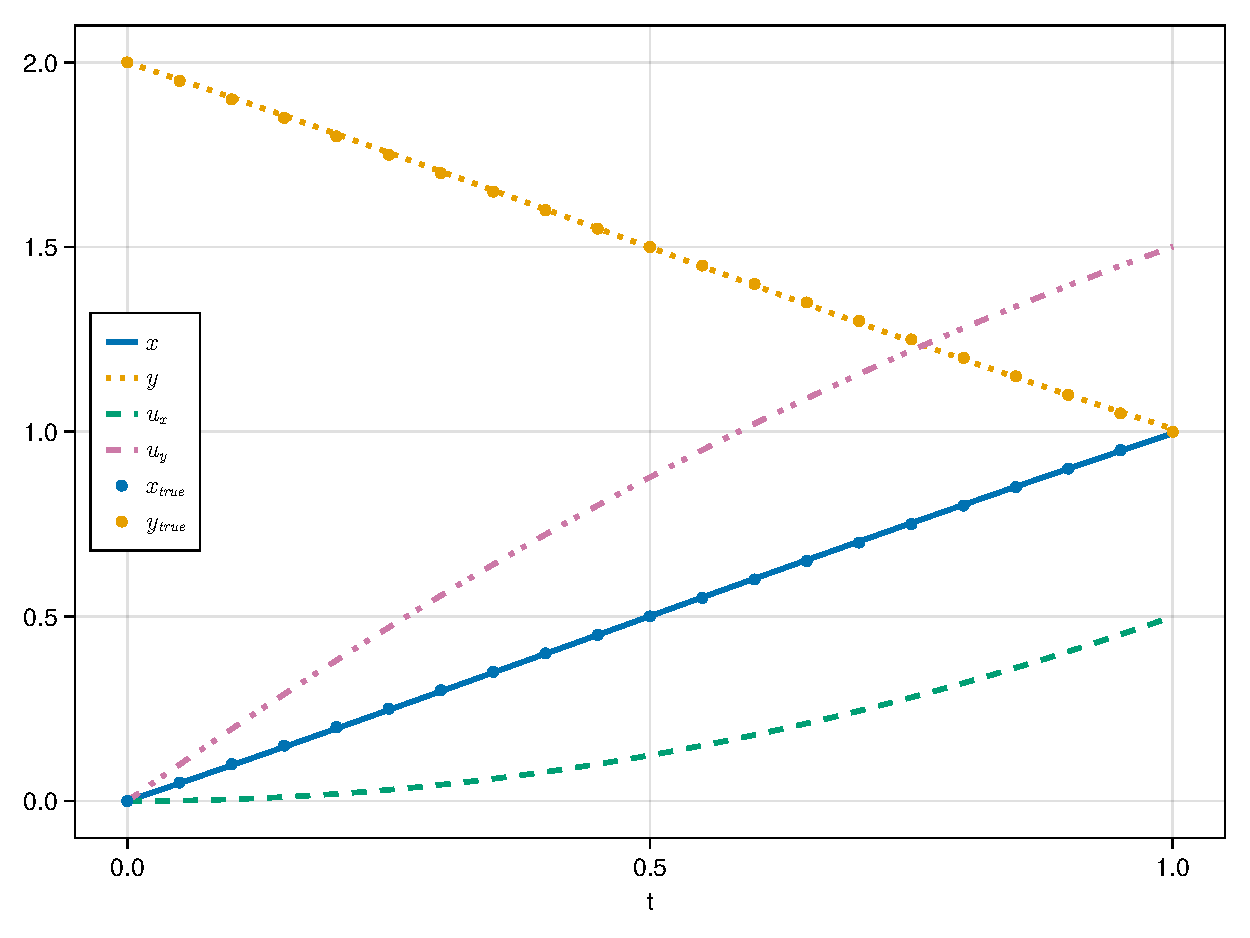
\includegraphics[width=0.8\textwidth]{../figures/lux/diffeq_plot.pdf}
  \caption{\textbf{Learning $2^{nd}$ order differential equation with Lux.jl.}}
  \label{fig:lux_diffeq_plot}
\end{figure}

\Cref{fig:lux_diffeq_plot} shows that our model is able to accurately learn the dynamics of the system from a few discrete data points. This is a very simple example, but it demonstrates the composability of Lux.jl and DifferentialEquations ecosystem.

\subsection{Gradient Free Optimization Algorithms}
\label{subsec:evolutionary_alg_lux}

Lux allows the parameters of a complicated neural network to be represented as a flattened vector. This allows it to interface directly with optimization packages without any glue code. In this example, we will train a neural network with gradient-free optimization algorithms to learn the function:
%
\begin{align}
  r(\theta)              & = e^{sin(\theta)} - 2cos(4\theta) + sin\left(\frac{2\theta - \pi}{12}\right)^5 \\
  \texttt{where } \theta & \in [0, 2\pi]
\end{align}
%
We will use algorithms implemented in packages that are agnostic to the specifics of Lux\footnote{Note that these are not the most efficient algorithms to solve the problem, but these simply demonstrate the composability of Lux.}:
%
\begin{itemize}
  \item Covariance Matrix Adaptation Evolutionary Strategy (CMAES)~\citep{hansen2016cma} from CMAEvolutionStrategy.jl.
  \item LN\_NEWUOA~\citep{powell2006newuoa} from NLopt.jl~\citep{johnson2021nlopt}. Since Lux allows flattened parameters we can easily interoperate with NLopt which is a C library.
\end{itemize}
%

\inputminted[linenos, breaklines, fontsize=\scriptsize, frame=single, framesep=10pt]{julia}{../code/gfopt.jl}

\begin{figure}[t]
  \centering
  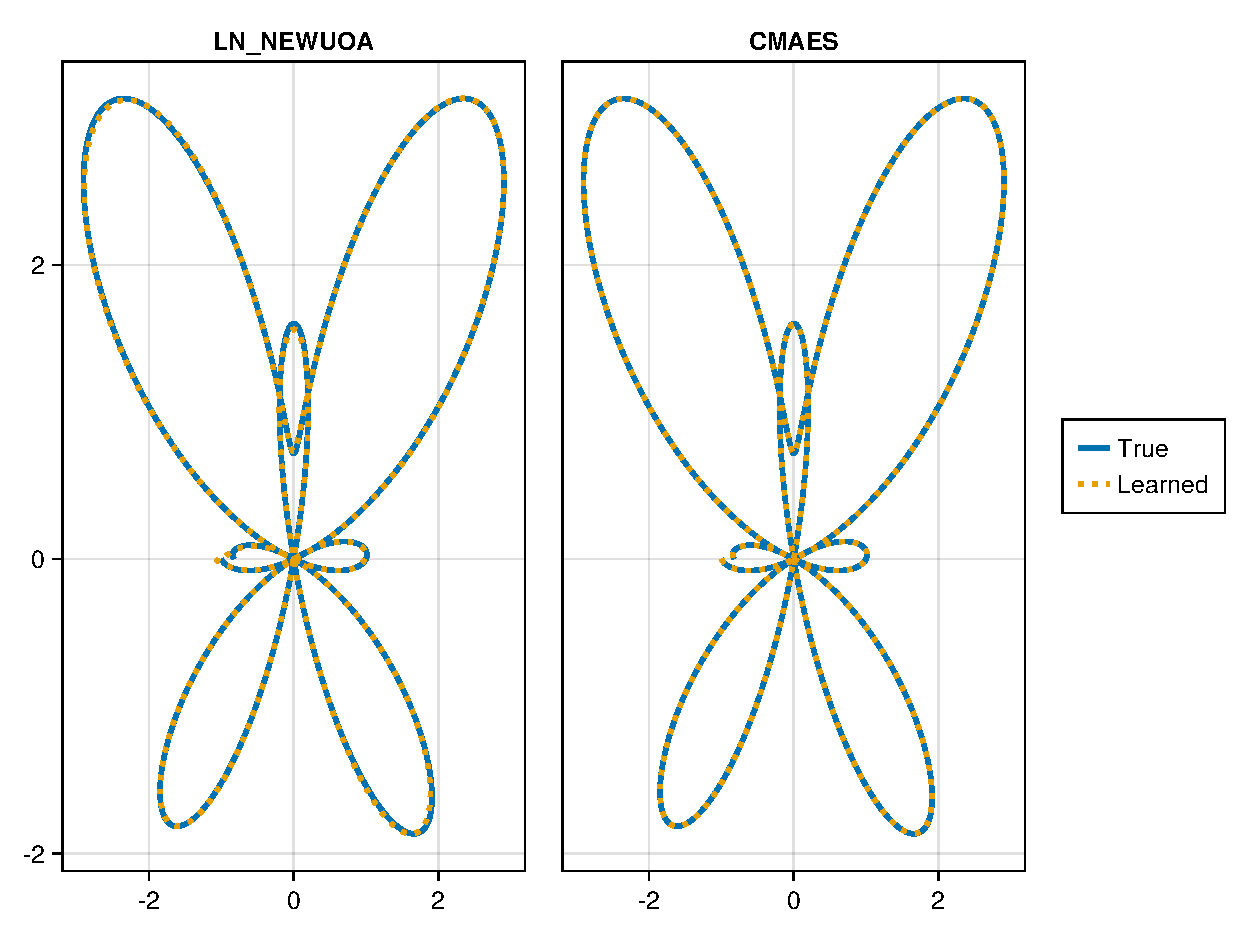
\includegraphics[width=\textwidth]{../figures/lux/gfopt_plot.pdf}
  \caption{\textbf{Gradient Free Optimization to train a neural network} to approximate the function $r(\theta) = e^{sin(\theta)} - 2cos(4\theta) + sin\left(\frac{2\theta - \pi}{12}\right)^5$.}
  \label{fig:lux_gfopt_plot}
\end{figure}

\subsection{Physics Informed Neural Networks}
\label{subsec:physics_informed_neural_networks_lux}

\todo{I want to showcase higher-order AD: not sure what example to use}

% In this section, we will describe how to model Physics-Informed Neural Networks (PINNs)~\citep{raissi2019physics} that leverage neural networks to solve Partial Differential Equations~(PDEs). 

% % \inputminted[linenos, fontsize=\footnotesize]{julia}{../code/pinn.jl}

% NeuralPDEs.jl~\citep{zubov2021neuralpde} extends Lux.jl to provide neural networks solvers for PDEs using PINNs.

% % \subsection{Higher Order Taylor Mode Automatic Differentiation}
% % \label{subsec:higher_order_taylor_mode_automatic_differentiation}

\subsection{Taylor Mode Automatic Differentiation}
\label{subsec:taylor_mode_automatic_differentiation}

\subsection{Combining Mixed Integer Programming with Neural Networks}
\label{subsec:combining_mixed_integer_programming_with_neural_networks}

% \section{Leveraging Cross-Language Capabilities}
% \label{sec:cross_language_capabilities}

% \todo{pycallchainrules for lux + pytorch and lux + jax}

\section{Performance}
\label{sec:performance_lux}

\todo{compare against flux and maybe knet}

\section{Discussion}
\label{sec:discussion_lux}

\subsection{Current Limitations}
\label{subsec:current_limitations}
